\section{Sheaves}
The central objects of study in this paper are \emph{sheaves}. At first
glance sheaves might seem complicated and abstract, but in fact they are
inherently geometric objects. Hence, I will not start with the
definition of sheaves, but instead I begin by discussing
\emph{fibre bundles}, which are more concrete objects that appear throughout 
geometry. This discussion should give a good motivation for
the definition of sheaves and also help build geometric intuition right
away.

\subsection{Motivation: fibre bundles}
The idea of a fibre bundle is to attach some space, called a \emph{fibre}
$F$, to every point of some topological space $B$, which will be called
the \emph{base space} \cite{hatcher}. When we attach the fibres to the
points of $B$, we should get a topological space $E$ called the
\emph{total space}. More formally, a fibre bundle consists of two spaces $E$
and $B$ and a continuous surjection (henceforth \emph{a projection})
$\pi:E\to B$, where the fibres $\pi^{-1}(b)$ of the projection are
homeomorphic to some fixed fibre space $F$. We require in addition
that one can find an open neighbourhood $U$ for every point of $B$ and a
homeomorphism $h:\pi^{-1}(U)\to U\times F$ such that the following diagram
commutes.
\begin{figure}[H]
  \centering
  \begin{minipage}{.45\textwidth}
    \centering
    \begin{tikzcd}[row sep=large, column sep=small]
      {\pi^{-1}(U)} && {U\times F} \\
      & U
      \arrow["\pi"', from=1-1, to=2-2]
      \arrow["{\text{proj}_1}", from=1-3, to=2-2]
      \arrow["h", leftrightarrow, from=1-1, to=1-3]
    \end{tikzcd}
  \end{minipage}%
  \begin{minipage}{.45\textwidth}
    \centering % TODO: Redo this picture
    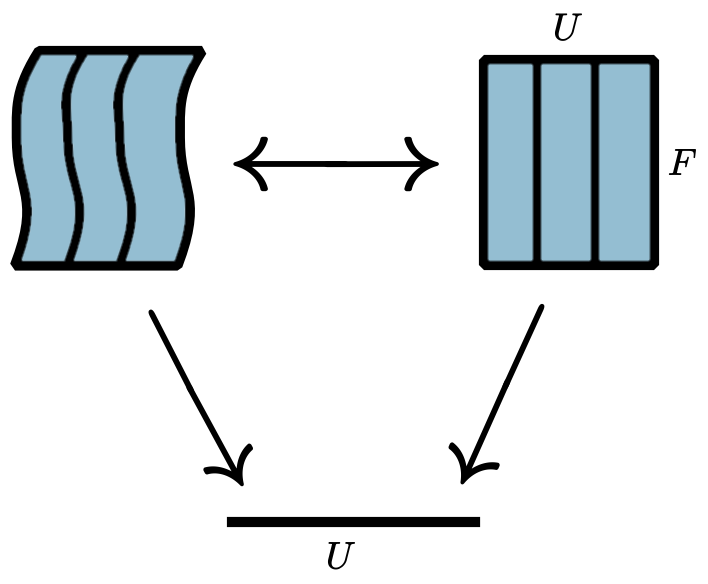
\includegraphics[width=.7\textwidth]{fibre_bundle}
  \end{minipage}
\end{figure}
Thus, when we attach the fibres to points of $B$, they should be gathered
so that the total space looks locally like a product space.

Let us look at some examples. Suppose the base space is the circle $S^{1}$
and the fibre space is the interval $(-1, 1)$, which is topologically
speaking a line. An example of such a \emph{line bundle} is the cylinder.
The cylinder is a \emph{trivial bundle}, because the total space can
be written as a product: $S^{1}\times (-1,1)$. An example of a
\emph{non-trivial line bundle} over $S^{1}$ is the \emph{Möbius strip}.
\begin{figure}[H]
  \centering
  \begin{minipage}{.45\textwidth}
    \centering
    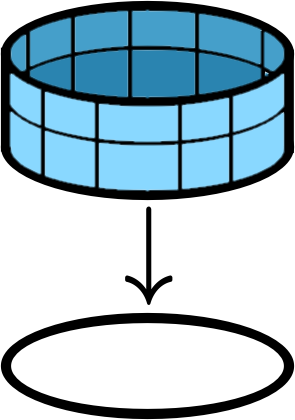
\includegraphics[height=4cm]{cylinder}
  \end{minipage}%
  \begin{minipage}{.45\textwidth}
    \centering
    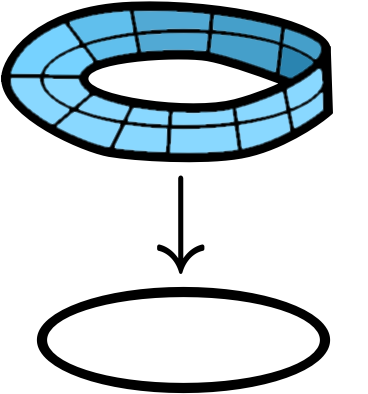
\includegraphics[height=4cm]{mobius}
  \end{minipage}
  \caption{The two line bundles over $S^{1}$}
\end{figure}
Similarly, we can consider \emph{circle bundles} over $S^{1}$. A trivial
circle bundle over $S^{1}$ is the torus and a non-trivial example is given
by the \emph{Klein bottle}.
An important example showing up in differential and algebraic geometry
is the concept of the \emph{tangent bundle}, where the fibres are the
tangent spaces at the points of the base space. Consider for example the
sphere $S^{2}$, which is a 2-dimensional manifold. Then the fibres of 
the tangent bundle of $S^{2}$ are the planes tangent to the sphere.

The things we are usually the most interested in are the \emph{sections} of
a given fibre bundle. A section $s$ of a fibre bundle $\pi:E\to B$
is a continuous map $s:B\to E$ such that $\forall b\in B,\ \pi(s(b))=b$.
This condition ensures that $s$ maps every point of the base space to the
corresponding fibre. A useful analogy is to think of a river, which can
be represented by a curve $C$ on the Euclidean plane. One could measure the
temperature of the river at different points and get a temperature reading
in $\mathbb{R}^{+}$ (assuming the
\begin{wrapfigure}{r}{0.3\textwidth} % TODO: Redo this picture
  \centering
  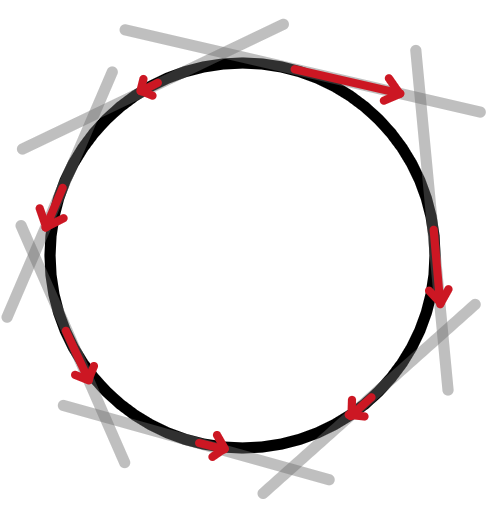
\includegraphics[width=0.3\textwidth]{vector_field}
  \caption{A section of the tangent bundle on $S^{1}$}
\end{wrapfigure}
 measurement is taken in Kelvins).
If one were to collect the temperature readings across all points of $C$,
one would get a section of the $\mathbb{R}^{+}$-bundle over the river $C$.
Thus, if fibre bundles are a way of attaching data to points of a space,
then sections of a fibre bundle are continuous collections of data over the
base space. Other interesting classes of examples of sections are vector
fields and differential forms, which are sections of the tangent bundle
and the cotangent bundle respectively. These are central objects of study
in geometry.

We often like to consider sections $s\vert_U:U\to E$ on some open set
$U\subseteq B$. These have the following property.
Given two sections $s_{1}:U_{1}\to E$ and $s_{2}:U_{2}\to E$, we can 
glue the two sections provided the sections
agree on $U_{1}\cap U_{2}$ to get a section $s:U_{1}\cup U_{2}\to E$.
Then, one can piece together larger sections from smaller sections. This
ability to define sections locally is very useful.

\subsection{Defining sheaves}
To summarise, fibre bundles are a way of attaching geometric data to
points of a given space, and one can consider sections over the fiber
bundle, which can be glued from small patches. We wish to extend the notion
of a fibre bundle, because the requirement that the fibres must be
topological spaces which form another topological space when bundled
together is more strict than we want.

The notion of a fibre bundle is extended by the notion of a sheaf.
Since taking sections is really the interesting part of fibre bundles, the
definition of a sheaf will not be built with fibres and projection maps
but with sections. For the rest of this section, I use \cite{gathmann} as
my main source for sheaf theoretic results. Next I will state the formal
definition of a \emph{pre-sheaf}. Pay attention to the properties that are
motivated by fibre bundles.
\begin{defin}
  A pre-sheaf $\mathscr{F}$ of sets on a topological space $X$ associates
  to each open set $U\subseteq X$ a set $\mathscr{F}(U)$, which is called
  the set of sections over $U$. For every pair of nested open sets
  $V\subseteq U$, one defines a function
  $\text{res}_{V}^{U}:\mathscr{F}(U)\to\mathscr{F}(V)$,
  called the restriction function, such that $\text{res}_{U}^{U}
  =\text{id}_{U}$ and for every triple $W\subseteq V\subseteq U$, we have
  $\text{res}_{W}^{V}\circ\text{res}_{V}^{U}=\text{res}_{W}^{U}$.
  For $s\in\mathscr{F}(U)$, one usually writes $s\vert_{V}$ for
  $\text{res}_{V}^{U}(s)$. Also, the set $\mathscr{F}(X)$ of global sections
  is denoted by $\Gamma(\mathscr{F})$.

  One can also define pre-sheaves of rings, for example, where the sets
  $\mathscr{F}(U)$ are rings and the restriction functions are
  ring homomorphisms.
\end{defin}
Note that pre-sheaves generalise the concept of taking sections on a
topological space, but this definition doesn't capture the important property
that sections should be able to be glued if they agree on the intersection.
Thus, sheaves are defined in the following way.
\begin{defin}
  A pre-sheaf $\mathscr{F}$ is a sheaf if the following property holds.
  Suppose $U\subseteq X$ is an open set with an open cover $(U_{i})_{i\in I}$.
  If $s_{i}\in\mathscr{F}(U_{i})$ are sections such that
  $s_{i}\vert_{U_{i}\cap U_{j}}=s_{j}\vert_{U_{i}\cap U_{j}}$ for all pairs $i$
  and $j$, then there is a unique section $s\in\mathscr{F}(U)$ such that
  $\forall i\in I,\ s\vert_{U_{i}}=s_{i}$.
\end{defin}
\begin{bcat}
  Category theoretically speaking, a pre-sheaf $\mathscr{F}$ of sets is
  simply a functor $\mathscr{F}:\text{Op}(X)^{\text{op}}
  \to\mathbf{Set}$, where $\text{Op}(X)$ is the posetal category of
  open sets of $X$. Moreover, a pre-sheaf of rings is a functor
  $\mathscr{F}:\text{Op}(X)^{\text{op}}\to \mathbf{Ring}$, and in general,
  a $\mathscr{C}$-valued pre-sheaf is a functor
  $\mathscr{F}:\text{Op}(X)^{\text{op}}\to\mathscr{C}$, where we define
  $\mathscr{F}(\emptyset)$ to be the final object of $\mathscr{C}$
  \cite{vakil}. If $\mathscr{C}$ has limits, we can also express the sheaf
  axiom category theoretically \cite{maclane}. Namely, $\mathscr{F}$ is a
  sheaf if for every open set $U$ of $X$ and an open cover $U_{i}$ of $U$ the
  following diagram is an equaliser diagram.
  \begin{equation}\label{diag:sheaf_eq}\begin{tikzcd}
      \mathscr{F}(U)\rar
      & \displaystyle\prod_{i}\mathscr{F}(U_{i})\rar[shift left]\rar[shift right]
      & \displaystyle\prod_{i,j}\mathscr{F}(U_{i}\cap U_{j})
    \end{tikzcd},\end{equation}
  where the first map is the product of the restrictions
  $\text{res}_{U_{i}}^{U}$ and the pair of maps are products of the
  restrictions $\text{res}_{U_{i}\cap U_{j}}^{U_{i}}$ and
  $\text{res}_{U_{i}\cap U_{j}}^{U_{j}}$ respectively.
\end{bcat}

Next, suppose $\pi: E\to B$ is a fibre bundle. One can easily check that
it is possible to define a sheaf $\mathscr{F}$ by
\[
  \mathscr{F}(U) = \Set{s:U\to E\mid s\text{ a section of }\pi}.
\]
An example of a sheaf showing up in algebraic geometry is the structure
sheaf $\mathscr{O}_{X}$ of an affine variety $X$ defined by
\[
  \mathscr{O}_{X}(U)=\Set{f\in k(X)\mid f\text{ regular on } U}.
\]
From now on, we will be concentrating on this sheaf more.

\subsection{Stalks and sheafification}
Now I will introduce two important constructions: stalks, which give a
zoomed-in picture of a sheaf, and sheafification, which turns pre-sheaves
into sheaves.

Suppose $\mathscr{F}$ is a pre-sheaf on some space $X$.
We would like to understand, what the structure of $\mathscr{F}$
is at some point $P$ by associating to the point a set $\mathscr{F}_P$ that describes this structure.
Since the only information specifying a pre-sheaf are the sections, we could define $\mathscr{F}_P$ to be
the set of sections over open sets containing $P$. However,
this is most often an unimaginably large a set. Thus,
we say that $\mathscr{F}_P$ is the set of equivalence classes
of such sections, where two sections are equivalent if they
agree on some sufficiently small open neighbourhood of $P$.
More formally:
\begin{defin}
  Given a pre-sheaf $\mathscr{F}$ on $X$ and a point $P\in X$, the stalk
  $\mathscr{F}_{P}$ at $P$ is defined as the set
  \[
    \mathscr{F}_{P}=\Set{(s, U)\mid U\subseteq X\text{ open}, P\in U, s\in
    \mathscr{F}(U)}/\sim,
  \]
  where two pairs $(s_{1}, U_{1})$ and $(s_{2}, U_{2})$ are equivalent
  if there is an open set $V\subseteq U_{1}, U_{2}$ containing $P$ such that
  \[
    s_{1}\vert_{V}=s_{2}\vert_{V}.
  \]
  The equivalence class of a pair $(s, U)$ is called the \emph{germ}
  of $s$ at $P$. Given a section $s\in\mathscr{F}(U)$, its germ at $P$
  is usually denoted by $s_{P}$.
\end{defin}
\begin{cat}
  The stalks can be written as the direct limit
  \[\mathscr{F}_{P}=\varinjlim_{U\ni P}\mathscr{F}(U).\]
\end{cat}
Next I will do an example computation with stalks, which will be useful
later.
\begin{prop}\label{prop:struct_stalk}
  Let $X$ be a variety. The stalk $\mathscr{O}_{X,P}$ of
  $\mathscr{O}_{X}$ at some point $P\in X$ is given by
  \[
    \mathscr{O}_{X,P}=\Set{\frac{f}g\in k(X)\mid f,g\in k[X],g(P)\neq 0}.
  \]
\end{prop}
\begin{proof}
  I will prove the two inclusions separately.
  \begin{description}[style=nextline]
    \item[$\subseteq\big)$]
          Let $[(\phi, U)]\in \mathscr{O}_{X,P}$. Since $P\in U$ and
          $\phi\in \mathscr{O}(U)$, $\phi$ must be regular at $P$. Thus,
          $\phi$ has a representation $\frac{f}g$ as a rational function
          around $P$, where $g(P)\neq 0$. Moreover, if $[(\phi_{1}, U_{1})]
          =[(\phi_{2}, U_{2})]$, then there is an open set $V\subseteq
          U_{1},U_{2}$ such that $\phi_{1}\vert_{V}=\phi_{2}\vert_{V}$.
          Therefore, $\phi_{1}$ and $\phi_{2}$ can be represented by the
          same rational function around $P$.
    \item[$\supseteq\big)$]
          Now suppose $\frac{f}g\in k(X)$ with $g(P)\neq 0$. Then, there
          is an open neighbourhood $U$ of $P$ where $g$ is non-zero.
          Clearly, $(\frac{f}g, U)$ defines a germ in $\mathscr{O}_{X,P}$.
  \end{description}
\end{proof}

The stalks of a sheaf are analogous to the fibres of a fibre bundle.
Just as a section of a fibre bundle takes values in the fibres, a section of
a sheaf takes values in the stalks.
\begin{lwarn}
  \begin{figure}[H]
    \begin{minipage}[t]{.5\textwidth}
      \vspace{0pt}
      Note however that while a stalk at $P$ contains all the data ``above''
      $P$ just as a fibre at $P$ does, stalks are larger, because they also
      contain local information \textbf{around} $P$. One can find two
      sections with equal values at $P$, but which have different germs at
      $P$.
    \end{minipage}%
    \begin{minipage}[t]{.45\textwidth}
      \centering
      \vspace{0pt}
      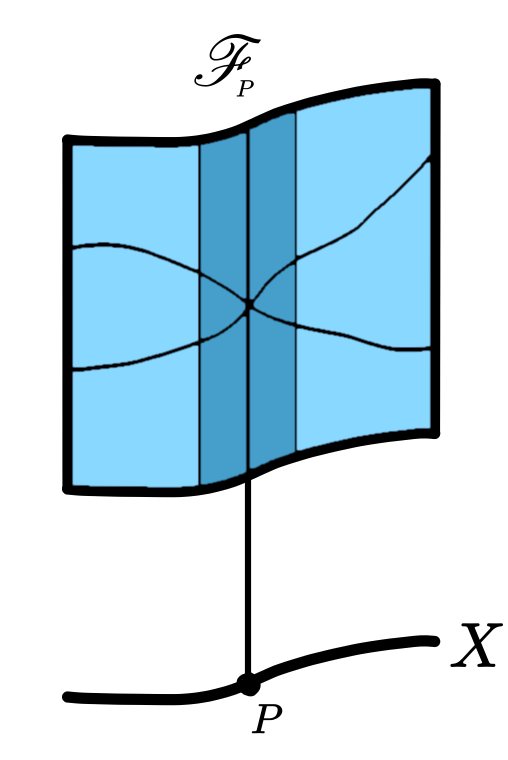
\includegraphics[width=.45\textwidth]{germs}
    \end{minipage}
  \end{figure}
\end{lwarn}
Next, we will study properties of germs that leads to the
construction of the sheafification of a pre-sheaf.
Fix a sheaf $\mathscr{F}$ on some space $X$ and choose a section
$s\in \mathscr{F}(U)$ on some open set $U\subseteq X$. Then, consider
the totality of germs of $s$ over $U$, namely the collection
$(s_{P})_{P\in U}$ with $s_{P}\in\mathscr{F}_{P}$. Since $\mathscr{F}$ is a
sheaf, it turns out that one can recover the section $s$ from the
germs: Each germ $s_{P}$ has a representative $(s\vert_{U_{P}}, U_{P})$.
The set $U$ is covered by the $U_{P}$ and since the $s\vert_{U_{P}}$ are
restrictions of the common section $s$ onto the sets $U_{P}$, one can use the
sheaf axiom to glue the sections $s\vert_{U_{P}}$ together and obtain a
section on $U$ which must be equal to $s$ by uniqueness. Generalising this
observation, one can write the sections of a sheaf as a collection of germs:
\begin{lemm}\label{lemm:sheafify_sheaf}
  Given a sheaf $\mathscr{F}$ on a space $X$, one can write
  \begin{align*}
    \mathscr{F}(U)=\big\{\,
    & (s_{P})_{P\in U}\,\big\vert\, s_{P}\in\mathscr{F}_{P}\text{ such that} \\
    & \forall P\in U\,
      \exists U_{P}\subseteq U\text{ an open neighbourhood of }P \\
    & \exists r\in\mathscr{F}(U_{P})\,\forall Q\in U_{P},\ r_{Q}=s_{Q}\,\big\}
  \end{align*}
  for every open set $U\subseteq X$
\end{lemm}
This statement may seem bewildering at first, but note that the important
part in the above observation was that when we fixed a point $P$, there was
an open set $U_{P}$ where all the germs $s_{Q}$ for $Q\in U_{P}$ agreed
with some section $s\vert_{U_{P}}$ on $U_{P}$. We want to ensure that this is
the case with the collection $(s_{P})_{P\in X}$ of the proposition so that we
can glue the germs in the same way as above. This statement will be essential
for building theory, but it is also useful for manipulating sheaves in
practise and I will routinely represent sections of sheaves as collections
of germs. Therefore, make sure you understand the statement and the proof
completely.
\begin{proof}
  I will again break up the proof into cases.

  \begin{description}[style=nextline]
    \item[$\subseteq\big)$]
          Suppose $s\in\mathscr{F}(U)$ is a section on $U$. Fix an arbitrary
          point $P\in U$ and choose a representative $(s\vert_{U_{P}}, U_{P})$
          of the germ $s_{P}$ of $s$. If one takes $r=s\vert_{U_{P}}\in
          \mathscr{F}(U_{P})$, then it follows immediately that
          \[\forall Q\in U_{P},\ r_{Q}=s_{Q}.\]
    \item[$\supseteq\big)$]
          Now, suppose $(s_{P})_{P\in U}$ is a collection of germs in the
          RHS set. Then, $U$ is covered by the sets $U_{P}$ associated to
          each germ $s_{P}$. Now, fix two points $P_{1},P_{2}\in U$,
          and consider the associated sections $r_{1}\in\mathscr{F}(U_{P_{1}})$
          and $r_{2}\in\mathscr{F}(U_{P_{2}})$. It is clearly the case that
          $r_{1}\vert_{U_{P1}\cap U_{P2}}=r_{2}\vert_{U_{P1}\cap U_{P2}}$, because
          of the germs of $r_{1}$ and $r_{2}$ are related through the germs
          $s_{P}$ on $U_{P_{1}}\cap U_{P_{2}}$. Therefore, we can take all
          the sections $r_{P}\in\mathscr{F}(U_{P})$ associated to the germs
          $s_{P}$ and glue them together to obtain a section $s$ on $U$.
          The germs of this section are clearly the germs $s_{P}$.
  \end{description}
\end{proof}

Now, since one can take stalks of pre-sheaves too, one might try this
construction on a pre-sheaf. If $\mathscr{F}^{\prime}$ is a pre-sheaf
on some space $X$, one can define another pre-sheaf $\mathscr{F}$
on $X$ by
\begin{align*}
  \mathscr{F}(U)=\big\{\,
  & (s_{P})_{P\in U}\,\big\vert\, s_{P}\in\mathscr{F}_{P}^{\prime}
    \text{ such that} \\
  & \forall P\in U\,
    \exists U_{P}\subseteq U\text{ an open neighbourhood of }P \\
  & \exists r\in\mathscr{F}^{\prime}(U_{P})\,\forall Q\in U_{P},
    \ r_{Q}=s_{Q}\,\big\}.
\end{align*}
Now, I leave it as an exercise for the reader to check that
$\mathscr{F}$ is in fact a sheaf. Thus, one can
associate a sheaf to every pre-sheaf using this construction, which is
called \emph{sheafification}.
\begin{rem}
  Note that Lemma~\ref{lemm:sheafify_sheaf} is saying that sheafifying a sheaf does 
  not do anything. One might also notice that this construction preserves 
  the stalks of $\mathscr{F}^{\prime}$, in other words, 
  $\mathscr{F}^{\prime}_{P}=\mathscr{F}_{P}$ for every $P\in X$. 
  This is true, because every element $(s, U)$ of $\mathscr{F}^{\prime}_{P}$ 
  can be associated to the element $(s_{Q})_{Q\in U}$ of $\mathscr{F}(U)$, 
  which in turn has a stalk at $P$ in $\mathscr{F}_{P}$ and an element 
  $((s_{Q})_{Q\in U},U)$ of $\mathscr{F}_{P}$ can be associated to 
  $s_{P}\in \mathscr{F}^{\prime}_{P}$.
\end{rem}
\begin{cat}
  The sheafification functor $\mathbf{PSh}(X)\to\mathbf{Sh}(X)$
  from the category of pre-sheaves on $X$ to the category of sheaves on $X$
  is the left adjoint to the forgetful functor $\mathbf{Sh}(X)\to
  \mathbf{PSh}(X)$ \cite{vakil}.
  In particular, there is a universal property defining the sheafification of a pre-sheaf.
\end{cat}
A typical example illustrating sheafification is to consider the constant
pre-sheaf and its sheafification. The constant pre-sheaf
$\mathscr{F}^{\prime}$ on a space $X$ is defined as follows
\[
  \mathscr{F}^{\prime}(U) =\Set{c: U\to\mathbb{R}\mid c
    \text{ a constant function }}.
\]
One can see that this is not a sheaf: take any two disjoint open sets
$U_{1}, U_{2}\subseteq X$ and two constant functions $c_{1}:U_{1}\to
\mathbb{R}$ and $c_{2}:U_{2}\to\mathbb{R}$ with different values.
Then, the two sections don't glue to form a constant function on
$U_{1}\cup U_{2}$ (all of this assumes that $X$ is a space with
at least one pair of disjoint open sets). The sheafification $\mathscr{F}$ of
$\mathscr{F}^{\prime}$ is given by sections $(c_{P})_{P\in U}$. By the
definition of sheafification, there is for every $P\in U$ an open
neighbourhood $U_{P}\subseteq U$ of $P$ and a constant function
$d: U_{P}\to\mathbb{R}$ such that $\forall Q\in U_{P},\ c_{Q}=d_{Q}$.
Hence, the restriction of $(c_{Q})_{Q\in U}$ to $U_{P}$ can be identified
with the constant function $d$. Therefore, the sheafification of the constant
pre-sheaf constists of \emph{locally constant functions}. In general, given
a set $A$, the constant sheaf $\underline{A}$ is defined as the sheafification
of the constant pre-sheaf with values in $A$.

Now is a good time to introduce other sheaves that will be needed later.
First one is the \emph{skyscraper sheaf} $A_P$ of some set $A$ at a point $P\in X$.
It is defined as follows
\[
  A_{P}(U)=\begin{cases}
    A, & \quad P\in U \\
    0, & \quad P\not\in U
  \end{cases}.
\]
What are the stalks of this sheaf at different points?

A second sheaf we need is the \emph{restriction sheaf} of some sheaf.
Suppose $\mathscr{F}$ is a sheaf on some space $X$ and $U\subseteq X$ is
an open set. Then, one defines the restriction sheaf $\mathscr{F}\vert_{U}$
on $U$ simply by
\[
  \mathscr{F}\vert_{U}(V)=\mathscr{F}(V)
\]
for open sets $V\subseteq U$.

\subsection{Ringed spaces and algebraic varieties}
Now that we have some feel for sheaves, I will briefly go over the
construction of abstract algebraic varieties, which are built with the help
of sheaves. Whenever I mention varieties, I refer to spaces that are
defined as in this subsection. The precise details of the construction are not
essential for the present article, and the reader should consult
\cite{gathmann} for a more detailed discussion.

In geometry, one is not only interested in the points of the space,
but also in the functions on the space. Thus, I will extend the notion of
a topological space by attaching the data of the functions on the space.
\begin{defin}
  A ringed space is a pair $(X,\mathscr{O}_{X})$ consisting of a topological
  space $X$ and a sheaf of rings $\mathscr{O}_{X}$ called the structure
  sheaf of $X$.
\end{defin}
Next, I will define morphisms between ringed spaces following the
definition given in \cite{gathmann}.
\begin{defin}
  Suppose $(X,\mathscr{O}_{X})$ and $(Y,\mathscr{O}_{Y})$ are two ringed
  spaces with structure sheaves consisting of $k$-valued functions
  for some field $k$. Then a morphism from $(X,\mathscr{O}_{X})$ to
  $(Y,\mathscr{O}_{Y})$ is a (set-theoretic) continuous map
  $f:X\to Y$ such that
  \begin{equation}\label{eq:ring_spc_morph}
    \forall U\subseteq Y\text{ open},\ f^{\ast}\mathscr{O}_{Y}(U)
    \subseteq \mathscr{O}_{X}(f^{-1}(U)),
  \end{equation}
  where $f^{\ast}g=g\circ f$ for $g\in\mathscr{O}_{Y}(U)$.
\end{defin}
To understand the condition in \eqref{eq:ring_spc_morph}, it helps to look
at the following commutative diagram.
\[\begin{tikzcd}[column sep=small]
    {X} && {Y} \\
    & k
    \arrow["{f^{\ast}g}"', from=1-1, to=2-2]
    \arrow["g", from=1-3, to=2-2]
    \arrow["f", from=1-1, to=1-3]
  \end{tikzcd}\]
The condition requires that functions $g\in\mathscr{O}_{Y}(U)$ ``pull back''
to functions in \linebreak $\mathscr{O}_{X}(f^{-1}(U))$ along the map $f:X\to Y$. As
usual, one can define isomorphisms of ringed spaces as morphisms
$f:(X,\mathscr{O}_{X})\to (Y,\mathscr{O}_{Y})$ such that there is a morphism
$g:(Y,\mathscr{O}_{Y})\to (X,\mathscr{O}_{X})$ with $f\circ g=g\circ f
=\text{id}$. Next I will define what it means for a ringed space to be
an affine variety.

\begin{defin}[Def. 2.3.15 in \cite{gathmann}]
  A ringed space $(X,\mathscr{O}_{X})$ is an affine variety if
  \begin{itemize}
    \item $X$ is an irreducible space,
    \item $\mathscr{O}_{X}$ is a sheaf of $k$-valued functions,
    \item There is an irreducible algebraic set $Y\subseteq \mathbb{A}^{n}$
          such that $(X,\mathscr{O}_{X})\cong (Y,\mathscr{O}_{Y})$.
  \end{itemize}
\end{defin}
Note that such ringed spaces are not always zero sets of some polynomials;
See for example Lemma 2.3.16 in \cite{gathmann}.

Now that I have defined what it means for a ringed space to be an affine
variety, I will form \emph{varieties} by ``gluing'' together open affine varieties
in the same way as manifolds are glued from open subsets of the Euclidean
space.
\begin{defin}[Def. 2.4.1 in \cite{gathmann}]
  A ringed space $(X,\mathscr{O}_{X})$ is a pre-variety if
  \begin{itemize}
    \item $X$ is an irreducible space,
    \item $\mathscr{O}_{X}$ is a sheaf of $k$-valued functions,
    \item $X$ can be covered with finitely many open sets $U_{i}$
          such that each $(U_{i},\mathscr{O}_{X}\vert_{U_{i}})$ is
          an affine variety.
  \end{itemize}
\end{defin}
The reason why we do not call these spaces varieties
is because the definition allows the construction of some pathological
spaces such as the \emph{line with two origins}, see \cite{gathmann}.
To avoid such spaces, we add one more condition in the final definition
of a variety. % TODO: Explain how the projective line is a variety
\begin{defin}[Def. 2.5.1 in \cite{gathmann}]
  A pre-variety $X$ is a variety, if for every pre-variety $Y$ and any
  pair of morphisms $f_{1}, f_{2}: Y\to X$, the set
  \[\set{P\in Y\mid f_{1}(P)=f_{2}(P)}\]
  is closed in $Y$.
\end{defin}
The following lemma will be needed later.
\begin{lemm}[Prop. 10.1.8 in \cite{vakil}]\label{lemm:affine_intersection}
  Suppose $X$ is a variety and $U, V\subseteq X$ are two open affine subsets.
  Then, the intersection $U\cap V$ is an open affine subset of $X$.
\end{lemm}
\begin{proof}
  Since the intersection of two open sets is open by definition,
  we need to only check that the intersection is affine.
  Recall that the product of two affine varieties is an
  affine variety, and consider the projection maps $\pi_U:U\times V\to U$
  and $\pi_V:U\times V\to V$. Also, denote by $\iota_U:U\to X$
  and $\iota_V:V\to X$ the inclusion maps. Then, we can see that
  \[
    U\cap V=\Set{P\in U\times V\mid (\iota_U\circ\pi_U)(P)=(\iota_V\circ\pi_V)(P)},
  \]
  which is closed, since $X$ is a variety.
  Therefore, the intersection is a closed subset of an
  affine variety.
\end{proof}

\subsection{Algebraic constructions with sheaves}\label{ss:sheaf_alg}
The aim of this subsection is to define algebraic constructions for
sheaves so that we can study them using the tools of
\emph{homological algebra}. First I need to define morphisms between
pre-sheaves.
\begin{defin}
  Suppose $\mathscr{F}$ and $\mathscr{G}$ are pre-sheaves of sets or rings
  on some space $X$. Then, a morphism $\alpha:\mathscr{F}\to\mathscr{G}$
  consists of set functions or ring homomorphisms
  $\alpha_{U}:\mathscr{F}(U)\to\mathscr{G}(U)$ which commute with restriction
  maps. That is, the following diagrams commute.
  \[\begin{tikzcd}
      \mathscr{F}(U)\rar{\text{res}_{V}^{U}}\arrow[d, "\alpha_{U}"']
      & \mathscr{F}(V)\dar{\alpha_{V}} \\
      \mathscr{G}(U)\arrow[r,"\text{res}_{V}^{U}"'] & \mathscr{G}(V)
    \end{tikzcd}\]
  Morphisms between sheaves are defined exactly the same way.
\end{defin}
One might ask, why this should be the right definition. The reason is that
this type of morphism \textbf{preserves the structure of the sheaf}. Compare
this with group homomorphisms. Firstly, a group homomorhism $\phi:G\to H$
associates to every element of $G$ a corresponding element in $H$. In the
same way a sheaf morphism $\alpha$ must associate to every section
$s\in\mathscr{F}(U)$ a corresponding section $\alpha_{U}(s)\in\mathscr{G}(U)$
of $\mathscr{G}$. Secondly, if three elements of the group are related by
the group structure so that $a\cdot b = c$, then the homomorphism should
respect this structure so that $\phi(a)\cdot\phi(b)=\phi(c)$. Similarly,
the sheaf morphism $\alpha$ should respect the structure of the sheaves
given by the restriction maps: if $s\vert_{V}=r$, then $\alpha(s)\vert_{V}
=\alpha(r)$.
\begin{cat}
  As one can immediately see, morphisms of pre-sheaves and sheaves are simply
  natural transformations of contravariant functors.
\end{cat}

In order to proceed to define algebraic constructions on sheaves, I must
restrict to some class of sheaves with an algebraic structure. The class
usually considered in algebraic geometry is the class of
\emph{sheaves of $\mathscr{O}_{X}$-modules} on a ringed space
$(X,\mathscr{O}_{X})$.
\begin{defin}
  Given a ringed space $(X,\mathscr{O}_{X})$, a sheaf $\mathscr{F}$ on $X$
  is a sheaf of $\mathscr{O}_{X}$-modules, if the sets $\mathscr{F}(U)$
  are $\mathscr{O}_{X}(U)$-modules and the restriction maps satisfy the
  following condition. Suppose $V\subseteq U\subseteq X$ are open and
  $s,s_{1}, s_{2}\in\mathscr{F}(U)$ are sections. Then,
  \[
    (s_{1}+s_{2})\vert_{V}=s_{1}\vert_{V}+s_{2}\vert_{V}\quad
    \text{and}\quad (\lambda s)\vert_{V}=\lambda\vert_{V}\cdot s\vert_{V}
  \]
  for all $\lambda\in\mathscr{O}_{X}(U)$.
\end{defin}
I can now define the usual algebraic operations for sheaves of
$\mathscr{O}_{X}$-modules.
\begin{defin}\label{def:sheaf_algebra}
  Suppose $\mathscr{F}_{1}$ and $\mathscr{F}_{2}$ are sheaves of
  $\mathscr{O}_{X}$-modules and $f:\mathscr{F}_{1}\to\mathscr{F}_{2}$ is a
  morphism of sheaves. Then the sheaves $\ker f$, $\coker f$,$\im f$,
  $\mathscr{F}_{1}\oplus\mathscr{F}_{2}$, $\mathscr{F}_{1}\otimes
  \mathscr{F}_{2}$, and $\mathscr{F}_{1}^{\vee}$ are defined as the
  sheafifications of the corresponding pre-sheaves given by the following:
  \begin{enumerate}
    \item $(\ker^{\prime} f)(U) = \ker(f_{U}:\mathscr{F}_{1}(U)
          \to\mathscr{F}_{2}(U))$
    \item $(\coker^{\prime} f)(U) = \coker(f_{U}:\mathscr{F}_{1}(U)
          \to\mathscr{F}_{2}(U))$
    \item $(\im^{\prime} f)(U)=\im(f_{U}:\mathscr{F}_{1}(U)
          \to\mathscr{F}_{2}(U))$
    \item $(\mathscr{F}_{1}\oplus^{\prime}\mathscr{F}_{2})(U)=\mathscr{F}_{1}(U)
          \oplus\mathscr{F}_{2}(U)$
    \item $(\mathscr{F}_{1}\otimes^{\prime}\mathscr{F}_{2})(U)
          =\mathscr{F}_{1}(U)\otimes_{\mathscr{O}_{X}(U)}\mathscr{F}_{2}(U)$
    \item $\mathscr{F}_{1}^{\vee\prime}(U)=\text{Hom}_{\mathscr{O}_{X}(U)}(
          \mathscr{F}_{1}(U),\mathscr{O}_{X}(U))$
  \end{enumerate}
\end{defin}
One can actually check that the pre-sheaves $\ker^{\prime} f$ and
$\mathscr{F}_{1}\oplus^{\prime}\mathscr{F}_{2}$ are in fact already sheaves,
so sheafification doesn't change the definition. We also have the following
usual definitions.
\begin{defin}\hfill

  \begin{enumerate}
    \item A morphism $f:\mathscr{F}_{1}\to\mathscr{F}_{2}$ of sheaves of
          $\mathscr{O}_{X}$-modules is injective if $\ker f = 0$ and
          surjective if $\coker f = 0$.
    \item If $f$ is injective, we write $\mathscr{F}_{2}/\mathscr{F}_{1}$
          for the cokernel.
    \item A sequence
          \[\begin{tikzcd}
              \cdots\rar & \mathscr{F}_{i-1}\rar & \mathscr{F}_{i}\rar
              & \mathscr{F}_{i+1}\rar & \cdots
            \end{tikzcd}\]
          of sheaves of $\mathscr{O}_{X}$-modules is exact if
          \[
          \ker(\mathscr{F}_{i}\to\mathscr{F}_{i+1})=\im(\mathscr{F}_{i-1}
          \to\mathscr{F}_{i}),\ \forall i.
          \]
  \end{enumerate}

\end{defin}
\begin{cat}
  One can show that the category $\mathscr{O}_{X}$\textbf{-Mod} of sheaves
  of $\mathscr{O}_{X}$-modules is an \emph{abelian category}, which means
  that it is a perfect setting for homological algebra (see \cite{vakil}).

  Furthermore, note that equaliser diagrams in abelian categories can be
  expressed in terms of exact sequences. Therefore, the sheaf axiom in
  \eqref{diag:sheaf_eq} can be expressed as the exact sequence
  \begin{equation}\label{diag:sheaf_ex}\begin{tikzcd}
      0\rar & \mathscr{F}(U)\rar
      & \displaystyle\bigoplus_{i}\mathscr{F}(U_{i})
      \rar{\text{res}_{U_{i}\cap U_{j}}^{U_{j}}-\text{res}_{U_{i}\cap U_{j}}^{ U_{i}}}
      &[5em] \displaystyle\bigoplus_{i,j}\mathscr{F}(U_{i}\cap U_{j})
    \end{tikzcd}\end{equation}
  in the category $\mathscr{O}_{X}$\textbf{-Mod} \cite{maclane}.
\end{cat}

Next I will show that the exactness of sequences of sheaves
is a local property. To see this, one should first note that a morphism
$f:\mathscr{F}_{1}\to\mathscr{F}_{2}$ of sheaves of
$\mathscr{O}_{X}$-modules induces an $\mathscr{O}_{X,P}$-module homomorphism
\[
  f_{P}:\left(\mathscr{F}_{1}\right)_{P}\to\left(\mathscr{F}_{2}\right)_{P}
  :[(s,U)]\mapsto [(f_{U}(s),U)]
\]
on the stalks. Then one can show the following theorem.
\begin{thm}[Lemma 13.21 in \cite{gathmann_new}]\label{thm:ses_equivalence}
  A sequence
  \[\begin{tikzcd}
      \cdots\rar{f_{i-2}} & \mathscr{F}_{i-1}\rar{f_{i-1}}
      & \mathscr{F}_{i}\rar{f_{i}} & \mathscr{F}_{i+1}\rar{f_{i+1}} & \cdots
    \end{tikzcd}\]
  of sheaves of $\mathscr{O}_{X}$-modules is exact if and only if the
  induced sequences
  \[\begin{tikzcd}
      \cdots\rar{\left(f_{i-2}\right)_{P}}
      & (\mathscr{F}_{i-1})_{P}\rar{\left(f_{i-1}\right)_{P}}
      & (\mathscr{F}_{i})_{P}\rar{\left(f_{i}\right)_{P}}
      & (\mathscr{F}_{i+1})_{P}\rar{\left(f_{i+1}\right)_{P}} & \cdots
    \end{tikzcd}\]
  on the stalks are all exact.
\end{thm}
\begin{proof}
  I will prove the two directions of the equivalence separately.
  \begin{description}[style=nextline]
    \item[$\Longrightarrow\big)$]
          The exactness of the first sequence implies
          that $\ker(f_{i})=\im(f_{i-1})$. Thus $\left(\ker(f_{i})\right)_{P}
          =\left(\im(f_{i-1})\right)_{P}$, and so
          \begin{align*}
            [(s, U)]\in\ker\left(\left(f_{i}\right)_{P}\right)
            &\iff \exists V\subseteq U,\ s\vert_{V}\in\ker^{\prime}(f_{i})(V)\\
            &\iff [(s\vert_{V},V)]\in\left(\ker(f_{i})\right)_{P} \\
            &\iff [(s\vert_{V},V)]\in\left(\im(f_{i-1})\right)_{P} \\
            &\iff \exists V\subseteq U,\ s\vert_{V}\in
              \im^{\prime}(f_{i-1})(V) \\
            &\iff [(s,U)]\in\im\left(\left(f_{i-1}\right)_{P}\right).
          \end{align*}
          Therefore, $\ker\left(\left(f_{i}\right)_{P}\right)
          =\im\left(\left(f_{i-1}\right)_{P}\right)$
          % TODO: Picture with exact sequence ker(f_i) -> F_i -> F_i+1
          %       and corresponding stalks
    \item[$\Longleftarrow\big)$]
          Choose an arbitrary open set $U\subseteq X$. Then,
          \begin{align*}
            s\in\ker(f_{i})(U)
            &\iff \forall P\in U,\ s_{P}\in\ker\left(\left(
              f_{i}\right)_{P}\right) \\
            &\iff \forall P\in U,\ s_{P}\in\im\left(\left(
              f_{i-1}\right)_{P}\right) \\
            &\iff s\in\im(f_{i-1})(U).
          \end{align*}
          In the first and the last equivalence one uses
          Lemma~\ref{lemm:sheafify_sheaf} to break the section $s$ into
          its germs and piece them back together. Thus,
          $\ker(f_{i})(U)=\im(f_{i-1})(U)$ for all open sets
          $U\subseteq X$, which implies that the sheaves are equal.
  \end{description}
\end{proof}
One can prove the following results as an immediate corollary.
\begin{cor}
  Suppose $f:\mathscr{F}\to\mathscr{G}$ is a morphism of sheaves of
  $\mathscr{O}_{X}$-modules, and let $f_{P}:\mathscr{F}_{P}\to\mathscr{G}_{P}$
  be the induced homomorphism. Then,
  \begin{enumerate}
    \item $f$ is an injection iff $f_{P}$ is an injection,
    \item $f$ is a surjection iff $f_{P}$ is a surjection,
    \item $f$ is an isomorphism iff $f_{P}$ is an isomorphism.
  \end{enumerate}
\end{cor}

In algebraic geometry, one further restricts attention to a certain class of
sheaves of $\mathscr{O}_{X}$-modules called \emph{quasi-coherent sheaves}.
These have even nicer algebraic properties, and they include most sheaves
one encounters in algebraic geometry. To define quasi-coherent sheaves,
I need to first make the following definition, which generalises the
definition of the structure sheaf on an affine variety.
\begin{defin}
  Suppose $X$ is an affine variety and $M$ is a module over the coordinate
  ring $\mathscr{O}_{X}(X)$. Then, the sheaf $\cm$ associated with the
  module $M$ is defined as follows.
  \begin{align*}
    \cm(U)=\big\{\,
    & (\phi_{P})_{P\in U}\,\big\vert\, \phi_{P}\in M_{\mathfrak{m}_{P}}
      \text{ such that} \\
    & \forall P\in U\,
      \exists U_{P}\subseteq U\text{ an open neighbourhood of }P \\
    & \exists m\in M\,\exists g\in \mathscr{O}_{X}(X)\,
    \forall Q\in U_{P},\ \phi_{Q}=\frac{m}g\,\big\},
  \end{align*}
  where $M_{\mathfrak{m}_{P}}$ is the localisation of $M$ at the maximal ideal
  $\mathfrak{m}_{P}$ of the point $P$.
\end{defin}
Now, this definition implies the following result.
\begin{lemm}\label{lemm:qcoh_local_global}
  If $\cm$ is the sheaf on an affine variety $X$ associated to the module
  $M$ over $\mathscr{O}_{X}(X)$, then
  \begin{enumerate}[label=\normalfont(\alph*)]
    \item $\forall P\in X, \left(\cm\right)_{P}=M_{\mathfrak{m}_{P}}$, and
    \item $\Gamma\left(\cm\right)=M$.
  \end{enumerate}
\end{lemm}
\begin{proof}
  The proof of part (a) is basically the same as the proof of
  Prop.~\ref{prop:struct_stalk}. Thus, I will only prove part (b) using
  ideas from the proof of Proposition 3.8 in \cite{gathmann_new}. Note
  that $M\subseteq\Gamma\left(\cm\right)$ holds trivially, and thus I
  only need to show $\Gamma\left(\cm\right)\subseteq M$.
  Begin by fixing an element $\varphi\in\Gamma\left(\cm\right)$.
  At a point $P\in X$, the section is represented by
  $\varphi_P=m_P/g_P$, where $m_P\in M$ and $g_P\in\mathscr{O}_X(X)$.
  Furthermore, $\varphi$ has this representation on an open neighbourhood $U_P$.
  
  Note first that the representations of $\varphi$ at
  any two points $P,Q\in X$ agree on the intersection
  $U_P\cap U_Q$. Since $X$ is an irreducible topological space,
  its non-empty open subsets are dense. Therefore, the
  intersection $U_P\cap U_Q$ is non-empty, and we have that
  \[g_Qm_P=g_Pm_Q\]
  for every pair of points $P,Q\in X$.

  Now, since $\varphi_P\in M_{\mathfrak{m}_P}$, we may assume $g_P(P)\neq 0$ for every $P\in X$.
  In particular, $P\not\in V(g_P)$. This implies that
  \[
    \bigcap_{P\in X}V(g_P)=\varnothing.
  \]
  By the Nullstellensatz, $\sqrt{(g_P\mid P\in X)}=(1)$, and therefore
  there are $k_P\in\mathscr{O}_X(X)$ such that
  \[1=\sum_{P\in I}k_Pg_P,\]
  where $I$ is some finite subset of $X$.
  If we set
  \[m=\sum_{P\in I}k_Pm_P,\]
  I claim that we can write $\varphi=m$ on the whole of $X$.
  Indeed, at a point $Q$, we have
  \[\varphi_Q=\frac{m_Q}{g_Q}=\frac{\sum_{P\in I}k_Pg_P\cdot m_Q}{g_Q}=\frac{\sum_{P\in I}k_Pg_Qm_P}{g_Q}=\sum_{P\in I}k_Pm_P=m.\]
  Therefore, we can conclude that $\varphi\in M$.
\end{proof}
Quasi-coherent sheaves are then constructed from such sheaves.
\begin{defin}
  A sheaf $\mathscr{F}$ of $\mathscr{O}_{X}$-modules is quasi-coherent, if
  for every affine open set $U\subseteq X$, the sheaf $\mathscr{F}\vert_{U}$
  is a sheaf associated to some module $M$ over the coordinate ring
  $\mathscr{O}_{X}(U)$.
\end{defin}
\begin{rem}
  To check quasi-coherence, it is enough to have an affine cover
  $(U_{i})_{i\in I}$, where $\mathscr{F}\vert_{U_{i}}$ is of the form $\cm$ for
  all $i\in I$, see \cite{gathmann}.
\end{rem}
\begin{rem}
  The constructios in Def.~\ref{def:sheaf_algebra} are quasi-coherent
  for quasi-coherent sheaves, see \cite{gathmann}.
\end{rem}
Quasi-coherent sheaves have the following nice property, which plays a
major role in the following section.
\begin{prop}[Lemma 7.2.7 in \cite{gathmann}]\label{prop:qcoh_gsec_exact}
  Given an affine variety $X$ and a short exact sequence
  \[\begin{tikzcd}
      0\rar & \cm_{1}\rar & \cm_{2}\rar & \cm_{3}\rar & 0
    \end{tikzcd}\]
  of quasi-coherent sheaves on $X$, the induced sequence
  \[\begin{tikzcd}
      0\rar & \Gamma(\cm_{1})\rar & \Gamma(\cm_{2})\rar
      & \Gamma(\cm_{3})\rar & 0
    \end{tikzcd}\]
  is exact.
\end{prop}
\begin{proof}
  By Lemma~\ref{lemm:qcoh_local_global}(b), I need to check the exactness of
  the sequence
  \[\begin{tikzcd}
      0\rar & M_{1}\rar & M_{2}\rar & M_{3}\rar & 0
    \end{tikzcd}.\]
  By a result in commutative algebra, this sequence is exact if the sequences
  \[\begin{tikzcd}
      0\rar & \left(M_{1}\right)_{\mathfrak{m}}\rar
      & \left(M_{2}\right)_{\mathfrak{m}}\rar
      & \left(M_{3}\right)_{\mathfrak{m}}\rar & 0
    \end{tikzcd}\]
  are exact for all maximal ideals $\mathfrak{m}$ of $k[X]$
  (see Proposition 6.27 of \cite{gathmann_comm}). Finally, combining
  Thm.~\ref{thm:ses_equivalence} with Lemma~\ref{lemm:qcoh_local_global}(a),
  we see that the sequences of the localisations are exact.
\end{proof}
